% Declare result floats before the study text to keep them close to the case studies.
\begin{figure*}[!t]
\centering
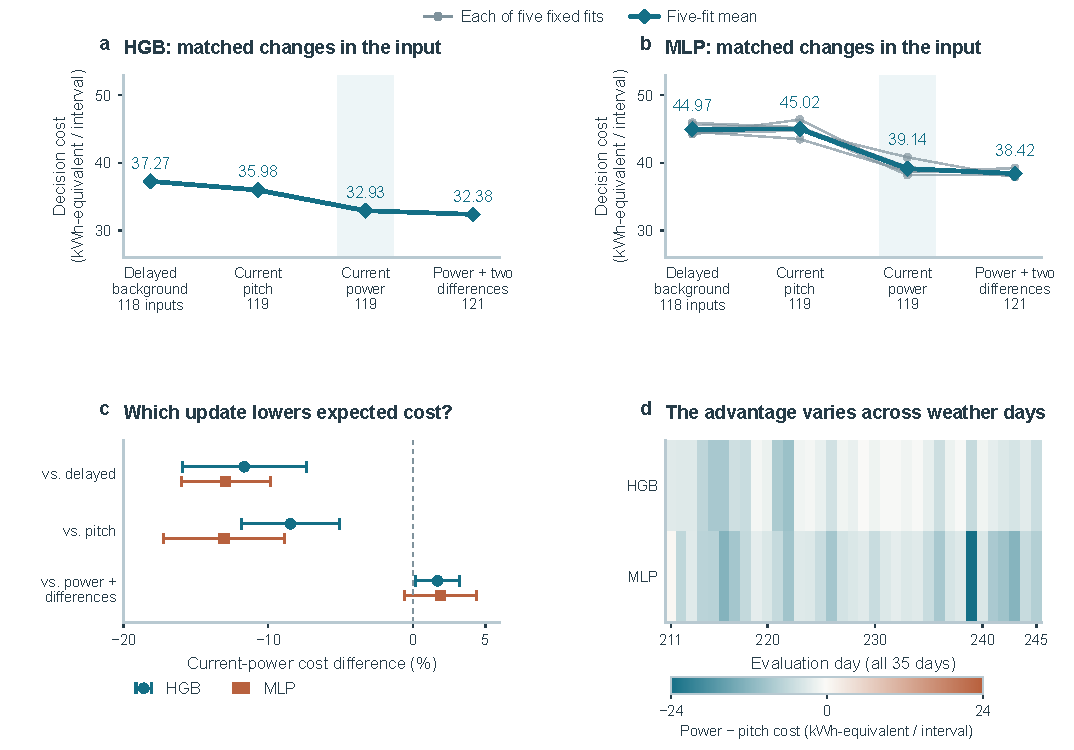
\includegraphics[width=\textwidth]{figures/v14/fig3_measurement.pdf}
\caption{The value of current measurements on a matched SDWPF population. (a), (b) Four input configurations share the same delayed background and evaluation rows. Thin lines connect each of the five fixed fits; diamonds and numbers show their means. Input counts include the four common inputs. (c) Relative current-power cost differences with stored approximate simultaneous 95\% intervals. Negative values favour current power. (d) Paired power-minus-pitch cost for every evaluation day, averaging the five fits. Blue denotes lower cost with power, and brown denotes higher cost. All 35 days and all 671,538 valid turbine intervals per fit are retained. The heatmap shows daily means.}
\label{fig:measurement}
\end{figure*}

\begin{figure*}[!t]
\centering
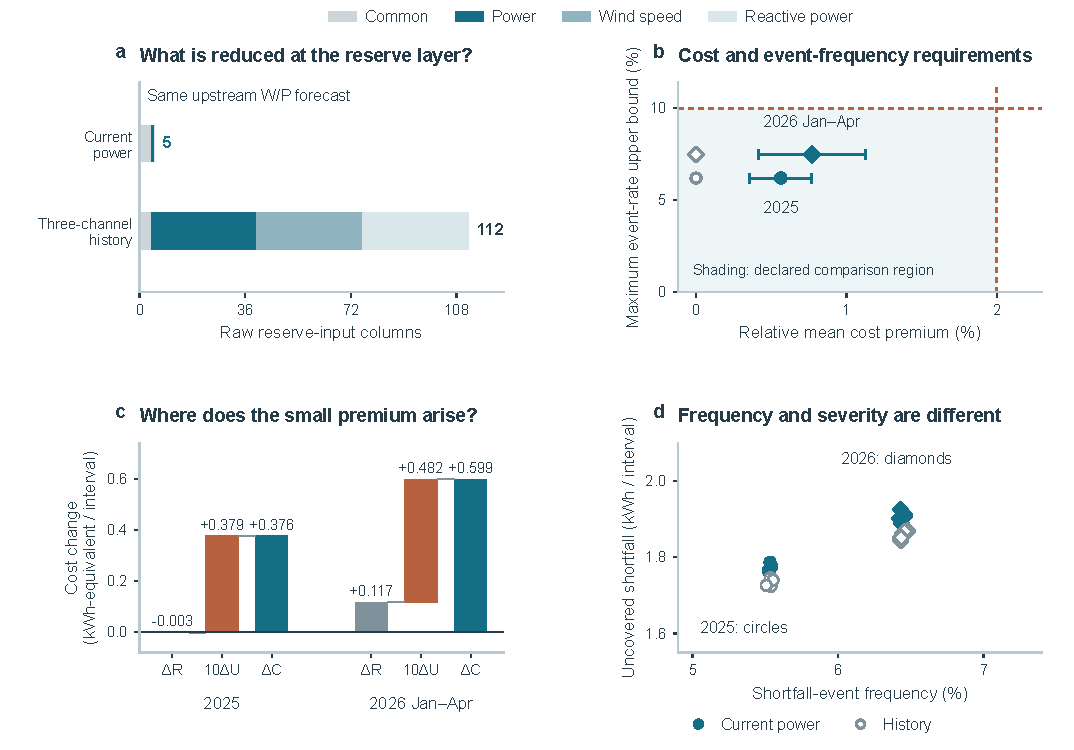
\includegraphics[width=\textwidth]{figures/v14/fig4_cross_year.pdf}
\caption{The cross-year trade-off from a compact reserve input. Both rules use HGB and $q=0.95$. (a) Input widths at the reserve layer, including four common inputs; the upstream forecast still uses wind-speed and power histories. (b) Filled markers show current-power relative mean cost and the maximum event-rate upper bound across five fits. Horizontal intervals are approximate simultaneous 95\% cost intervals. Open markers show the corresponding reference event bounds at zero self-relative cost. The shaded region marks the 2\% cost margin and 10\% event cap; years have separate inference families. (c) The cost premium decomposes as $\Delta C=\Delta R+10\Delta U$. The middle waterfall bar starts at $\Delta R$, and the final bar shows the total. (d) All five fit endpoints for each rule and period show event frequency alongside uncovered-shortfall magnitude. These points are descriptive, not confidence bounds.}
\label{fig:crossyear}
\end{figure*}

\begin{figure*}[!t]
\centering
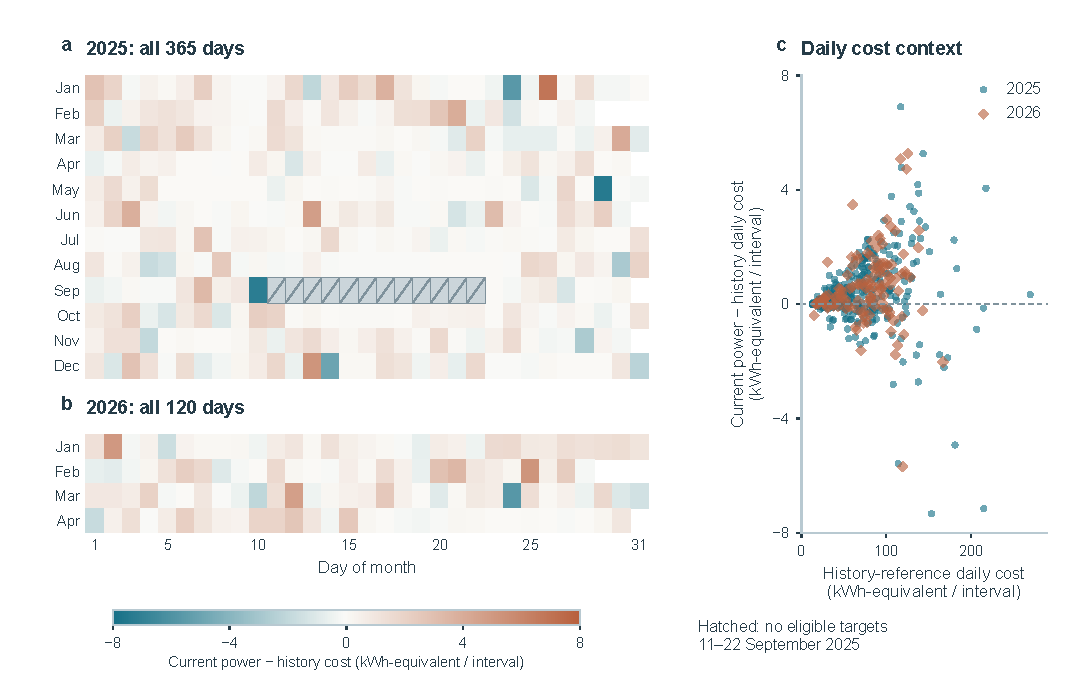
\includegraphics[width=\textwidth]{figures/v14/fig5_temporal.pdf}
\caption{Daily cost differences across the complete evaluation calendars. (a), (b) Each calendar cell shows the five-fit mean paired cost difference, current power minus history, using the same colour scale. Blue favours current power and brown favours history. All 365 dates in 2025 and 120 dates in January--April 2026 are retained. Gray cells with diagonal marks denote 11--22 September 2025, when no eligible targets were recorded; blank cells beyond a month's final day are not dates. (c) All valid daily differences are plotted against the reference's daily cost. These descriptive day-level views retain heterogeneous outcomes; window-level estimates pool valid-record numerators and denominators, with uncertainty reported in Fig.~\ref{fig:crossyear}.}
\label{fig:temporal}
\end{figure*}
